\subsection{Passage du modèle Entité-Association au modèle relationnel}
Nous avions pour consigne d'utiliser un schéma Entité-Association précis et de réaliser le modèle relationnel correcpondant.

\begin{figure}
	\begin{center}
	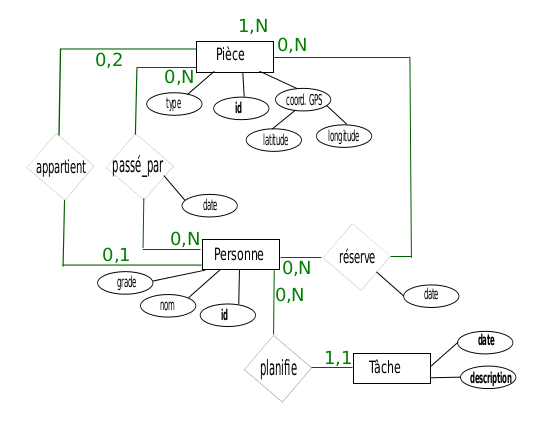
\includegraphics[width=500px]{./images/SchemaEA.png}
	\end{center}
\caption{Schéma EA}
\label{Schéma EA}
\end{figure}

En suivant chaque étape du cours, nous avons obtenu les résultats suivants :

\begin{enumerate}
	\item Passage des entités en relations:
		\begin{itemize}
			\item PIECE(idPiece, type, lattitude, longitude) : l'attribut composite coord\_GPS est remplacé par ces 2 attributs, lattitude et longitude.
			\item PERSONNE(id, nom, grade)
			\item TACHE(date, tache) 
		\end{itemize}
	\item Passage des entités faibles en relations : rien à faire puisqu'il n'y a pas d'entités faibles
	\item Association binaire 1,1 par clé étrangères :
		\begin{itemize}
			\item PIECE(idPiece, type, lattitude, longitude)
			\item PERSONNE(id, nom, grade)
			\item TACHE(date, tache, id) : on ajoute la clé étrangère id, clé de PERSONNE car il y a une cardinalité 1,1
		\end{itemize}
	\item Assocations binaires M,N :
		\begin{itemize}
			\item PIECE(idP, type, lattitude, longitude)
			\item PERSONNE(idPers, nom, grade)
			\item TACHE(date, tache, idPers)
			\item APPARTIENT(idP, idPers) : Création de la relation APPARTIENT à cette étape
			\item PASSEPAR(idP, idPers, date) : Création de la relation PASSEPAR à cette étape
			\item RESERVATION(idP, idPers, date) : Création de la relation RESERVATION à cette étape
		\end{itemize}
	\item Il n'y a pas d'attributs multi-valués ni d'association n-aire.
\end{enumerate}

\subsection{Critique du modèle proposé}
